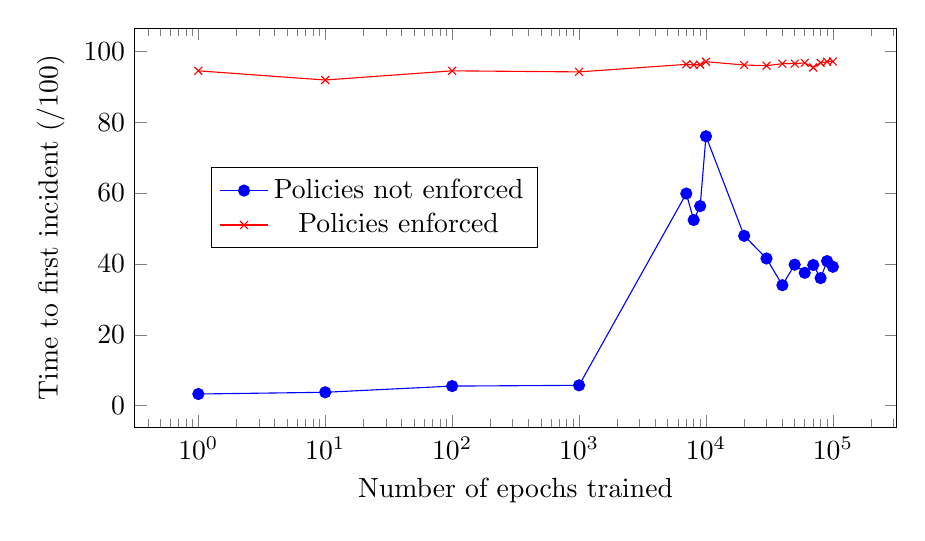
\begin{tikzpicture}
\begin{semilogxaxis}[
xlabel={Number of epochs trained},
ylabel={Time to first incident (/100)},
x=0.7cm,
y=0.45mm, 
legend style={at={(0.1,0.55)},anchor=west}]

\addplot[color=blue,mark=*] coordinates {
	(0, 3.24)
	(1, 3.29)
	(10, 3.78)
	(100, 5.53)
	(1000, 5.74)
	(7000, 59.87)
	(8000, 52.39)
	(9000, 56.33)
	(10000, 76.03)
	(20000, 47.94)
	(30000, 41.54)
	(40000, 34)
	(50000, 39.8)
	(60000, 37.5)
	(70000, 39.7)
	(80000, 36)
	(90000, 40.8)
	(100000, 39.2)
};

\addplot[color=red,mark=x] coordinates {
	(0, 93.2)
	(1, 94.5)
	(10, 91.91)
	(100, 94.5)
	(1000, 94.2)
	(7000, 96.33)
	(8000, 96.21)
	(9000, 96.24)
	(10000, 97.07)
	(20000, 96.15)
	(30000, 95.94)
	(40000, 96.52)
	(50000, 96.53)
	(60000, 96.74)
	(70000, 95.44)
	(80000, 96.75)
	(90000, 97.09)
	(100000, 97.14)
};

\legend{Policies not enforced, Policies enforced}
\end{semilogxaxis}%
\end{tikzpicture}%